%% 
%% This is file, `3b.tex',
%% generated with the extract package.
%% 
%% Generated on :  2019/02/03,13:04
%% From source  :  main.tex
%% Using options:  active,generate=3B.tex,extract-env={boehm}
%% 
\documentclass{article}

\begin{document}

\begin{boehm}

\section{Introduction}

The goal of this section is to characterize the statistical power of our pleiotropy test under a variety of conditions by studying a real data set. We examine pancreatic islet expression traits from the \citet{keller2018genetic} data. As in chapters 2 and 3A, we test only two traits at a time. Because we’ve chosen local expression traits in our analysis, we both know where each trait’s true QTL location (approximately), and we anticipate that each trait has a unique QTL that is distinct from QTL for other local expression traits. This design thus provides opportunities to study statistical power for our test.

We anticipate that inter-locus distance, univariate QTL strength, and correlation of founder allele effects patterns are three factors that contribute to power for our test. Specifically, we expect that greater inter-locus distance, greater univariate LOD scores, and less similar founder allele effects patterns correspond to greater statistical power to detect two separate QTL.

We use pancreatic islet gene expression traits from a publicly available data set, which \citet{keller2018genetic} first collected, analyzed, and shared. We examine a collection of 80 local traits on Chromosome 19 and perform our test for pleiotropy on pairs of traits. We also examine pairwise relationships among gene expression traits to characterize the impacts of univariate LOD score, inter-locus distance, and similarity of founder allele effects patterns on pleiotropy test statistics.



\section{Methods}


We analyzed data from 378 Diversity Outbred mice \citep{keller2018genetic}. \citet{keller2018genetic} genotyped tail biopsies with the GigaMUGA microarray \citep{morgan2016mouse}. They used RNA sequencing to measure genome-wide pancreatic islet cell gene expression for each mouse at the time of sacrifice \citep{keller2018genetic}. They shared these data, together with inferred founder allele probabilities, on the Data Dryad site (\url{https://datadryad.org/resource/doi:10.5061/dryad.pj105}). We performed analyses with the R statistical computing environment \citep{r} and the packages \texttt{qtl2} \citep{qtl2} and \texttt{qtl2pleio} \citep{qtl2pleio}.


We study below 80 Chromosome 19 local expression QTL and their corresponding transcript levels. We define a local expression QTL to be an expression QTL that is on the same chromosome as the gene itself. For example, the \emph{Asah2} gene is located on Chromosome 19 and its transcript levels have an expression QTL on Chromosome 19 (Table \ref{tab:ann4}). Thus, we term the Chromosome 19 \emph{Asah2} expression QTL a local expression QTL.

We choose to focus on local expression QTL, while ignoring nonlocal expression QTL, because we know, approximately, the true locations for local expression QTL. That is, a local expression QTL is near the corresponding gene position. Additionally, we expect that a given local expression QTL affects only one local expression trait. In our example above, we expect that the \emph{Asah2} expression QTL is near the \emph{Asah2} gene position and that no other local expression traits map to it.


Our design involves selection of a set of ``anchor'' expression traits. Gene \emph{Asah2} is located near the center of Chromosome 19 and has a very strong local expression QTL (Table \ref{tab:ann4}). We chose it as our first ``anchor'' gene expression trait. To diversify our collection of anchor genes, we chose three additional expression traits with local expression QTL. These three are \emph{Lipo1}, \emph{Lipo2}, and \emph{4933413C19Rik} (Table \ref{tab:ann4}). Together, the four anchor genes represent a variety of strong local expression trait LOD scores (from 60 to 101) and demonstrate modest variability in their founder allele effects (Table~\ref{tab:effects}). All four anchor genes are located near the middle of Chromosome 19 (Table~\ref{tab:ann4}).




We identified a set of 76 non-anchor local expression traits that map to the 20-Mb region centered on the peak for \emph{Asah2}, at 32.1 Mb. Each trait among the 76 maps to Chromosome 19 with a univariate LOD score of at least 10 (Table \ref{tab:ann76}).


% latex table generated in R 3.5.2 by xtable 1.8-3 package
% Thu Jan  3 16:29:15 2019
\begin{table}[ht]
\caption{Annotations for four anchor genes.}\label{tab:ann4}
\centering
\begin{tabular}{>{\em}lrrrr}
  \hline
symbol & start & end & peak\_position & lod \\
  \hline
Asah2 & 31.98 & 32.06 & 32.14 & 101.20 \\
  Lipo1 & 33.52 & 33.76 & 33.67 & 85.46 \\
  Lipo2 & 33.72 & 33.76 & 33.02 & 77.21 \\
  4933413C19Rik & 28.58 & 28.58 & 28.78 & 60.41 \\
   \hline
\end{tabular}
\end{table}







For each Chromosome 19 marker, we estimated founder allele and covariate effects. We calculated:

\begin{equation}\label{eq:uni-Bhat}
\widehat {(B:C)} = \left((X:W)^T\hat\Gamma^{-1}(X:W)\right)^{-1}(X:W)^T\hat\Gamma^{-1}Y
\end{equation}

\noindent where $B:C$ denotes the concatenation of $B$ and $C$, and $X:W$ refers to the $n$ by $12$ matrix resulting from appending the columns of $W$ to the $X$ matrix. $\hat\Gamma$ is the covariance matrix defined by Equation \ref{eq:Sigma}.

\begin{equation}\label{eq:Sigma}
\hat \Gamma = \hat\sigma_g^2 K + \hat \sigma_e^2 I_n
\end{equation}

\noindent We denote the restricted maximum likelihood estimates of the variance components by $\hat \sigma_g^2$ and $\hat \sigma_e^2$.


For each of the 80 expression traits, we calculated fitted values for each subject with the estimated founder allele and covariate effects (Equation \ref{eq:uni-Bhat}). We then calculated correlations between fitted values for pairs of traits. Each pairing involved one anchor gene expression trait and one other gene expression trait.

We anticipated that more similar two traits' founder allele effects would correspond, on average, to smaller pleiotropy test statistics. We base this expectation on findings from \citet{macdonald2007joint} and \citet{king2012genetic}. \citet{macdonald2007joint} and \citet{king2012genetic} found that two traits that associate with a single pleiotropic QTL tended to have similar founder allele effects patterns for biallelic markers.

We performed two-dimensional QTL scans for $4 * 76 + \binom{4}{2} = 310$ pairs. Each pair included one of the four anchor gene expression traits and either one of 76 non-anchor gene expression traits or one of the remaining three anchor gene expression traits.

Our two-dimensional QTL scan encompassed a 1000 by 1000 marker grid from 18.1 Mb to 42.5 Mb on Chromosome 19. Each scan involved fitting 1000 x 1000 = 1,000,000 models via generalized least squares. For a given ordered pair of markers, we used the bivariate linear mixed effects model and methods defined in Chapter 2. These methods are implemented in the R package \texttt{qtl2pleio} \citep{qtl2pleio}.

For each of the 80 expression traits, we used the fitted founder allele and covariate effects ($\widehat{B:C}$ in Equation~\ref{eq:uni-Bhat}) to obtain fitted values vectors for every subject and all 80 traits (Equation~\ref{eq:fitted}). For each of the 310 pairings of traits, we calculated correlations among the fitted values vectors. Our motivation for working with the fitted values vectors (instead of the $\hat B$ estimated founder allele effects vectors) is that the fitted values approximately weight the allele effects by allele frequency. An alternative analysis might neglect the covariates when calculating fitted values.

\begin{equation}\label{eq:fitted}
\hat Y = X\hat B + W \hat C
\end{equation}


\section{Results}

% latex table generated in R 3.5.2 by xtable 1.8-3 package
% Sat Feb  2 10:17:32 2019
\begin{table}[ht]
\caption{Founder allele effect estimates at Chromosome 19 QTL peak position.}\label{tab:effects}
\centering
\begin{tabular}{>{\em}cccc}
  \hline
 Gene Symbol & Founder allele & Effect & Standard error \\
  \hline
\multirow{8}{*}{Asah2} & A & -0.96 & 0.17 \\
  & B & 1.01 & 0.19 \\
  & C & 0.14 & 0.17 \\
  & D & -1.16 & 0.17 \\
  & E & 1.05 & 0.16 \\
  & F & -0.61 & 0.20 \\
  & G & 1.81 & 0.16 \\
  & H & -0.18 & 0.18 \\
  \hline
  \multirow{8}{*}{Lipo1} & A & 0.29 & 0.18 \\
  & B & 0.13 & 0.21 \\
  & C & 0.28 & 0.20 \\
  & D & 0.23 & 0.19 \\
  & E & -0.17 & 0.18 \\
  & F & -0.28 & 0.21 \\
  & G & 2.55 & 0.19 \\
  & H & -0.72 & 0.19 \\
  \hline
\multirow{8}{*}{Lipo2} & A & -0.10 & 0.18 \\
  & B & -0.28 & 0.23 \\
  & C & 0.00 & 0.20 \\
  & D & 0.01 & 0.18 \\
  & E & -0.77 & 0.17 \\
  & F & -0.89 & 0.22 \\
  & G & 2.65 & 0.18 \\
  & H & -0.70 & 0.20 \\
   \hline
\multirow{8}{*}{4933413C19Rik} & A & 0.29 & 0.23 \\
  & B & 0.76 & 0.24 \\
  & C & 0.81 & 0.21 \\
  & D & 0.49 & 0.24 \\
  & E & 0.67 & 0.20 \\
  & F & -0.53 & 0.22 \\
  & G & -1.65 & 0.18 \\
  & H & 0.67 & 0.21 \\
   \hline
\end{tabular}
\end{table}


All four anchor traits demonstrate strong PWK (``G'') allele effects. \emph{Lipo2} and \emph{Asah2} have similar patterns among allele effects (at their respective QTL peaks) (Table~\ref{tab:effects}).


%\subsection{Pleiotropy likelihood ratio test statistic vs. chromosomal position}

\begin{figure}
    \centering
    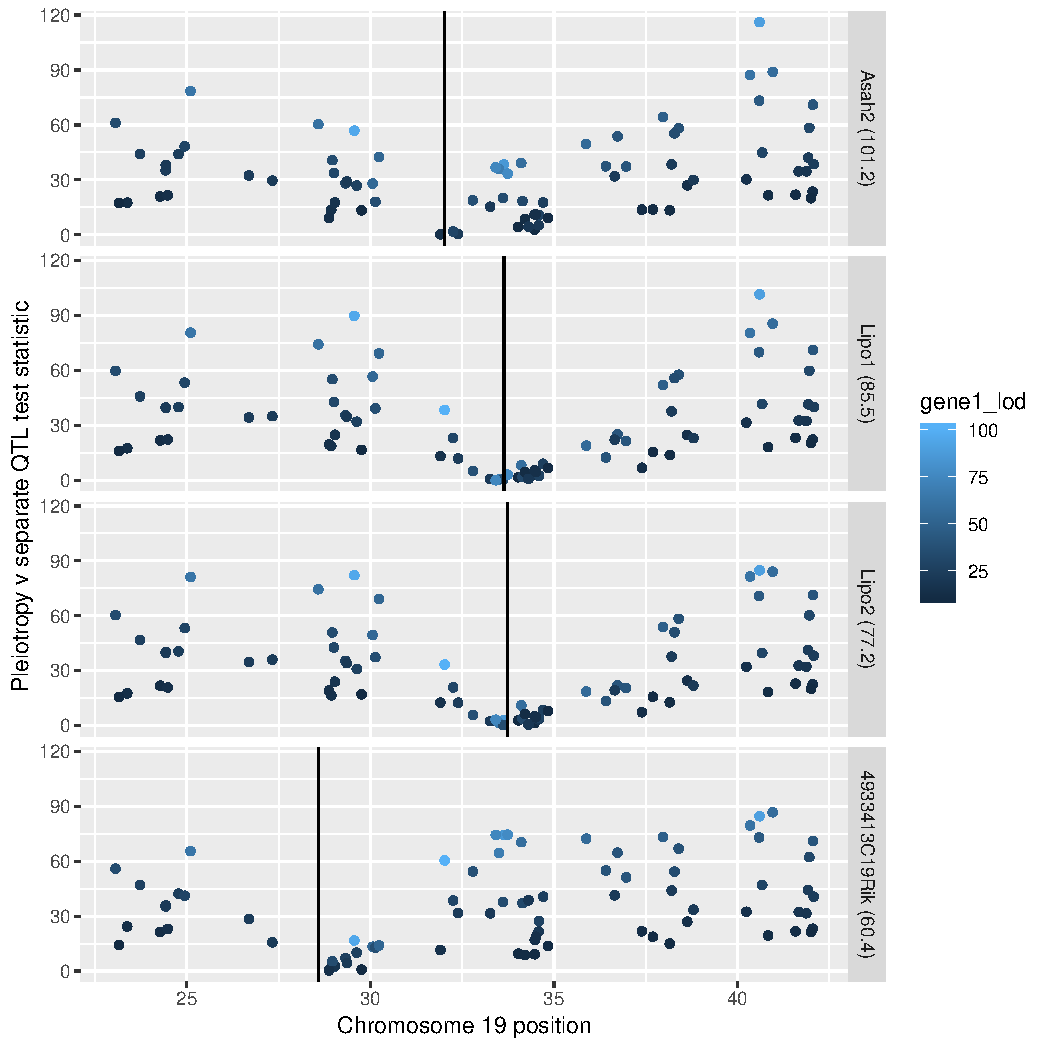
\includegraphics[width = \textwidth]{../Rmd/lrt-v-middle-of-gene.pdf}
    \caption[Pleiotropy LRT vs. chromosomal position plots reveal that higher values of pleiotropy LRT tend to correspond to greater interlocus distance and greater univariate LOD score.]{Each anchor gene has its own panel. Along the horizontal axis is Chromosome 19 position. The vertical axis is for pleiotropy test statistic value. Each point corresponds to a local gene expression trait. Point color corresponds to the nonlocal gene's univariate LOD score, with lighter shades of blue denoting greater values of univariate LOD score. Vertical black bar denotes the anchor gene's position on Chromosome 19. All four panels reveal that points further from the anchor gene tend to show greater test statistic values. Additionally, the Lipo1 and Lipo2 panels offer an opportunity to compare the impact of anchor gene univariate LOD score on pleiotropy test statistic values.}
    \label{fig:middle}
\end{figure}

Each anchor gene has its own panel in Figure \ref{fig:middle}. Along the horizontal axis is Chromosome 19 position. The vertical axis is for pleiotropy test statistics. Each point corresponds to a local gene expression trait. Point color corresponds to the nonlocal gene's univariate LOD score, with lighter shades of blue denoting greater values of univariate LOD score. Vertical black bar denotes the anchor gene's position on Chromosome 19. All four panels reveal that points further from the anchor gene tend to show greater test statistic values. Additionally, because of their nearly identical positions, the \emph{Lipo1} and \emph{Lipo2} panels offer an opportunity to compare the impact of anchor gene univariate LOD score on pleiotropy test statistics.




%\subsection{Pleiotropy likelihood ratio test statistics vs. univariate LOD scores}

\begin{figure}
    \centering
    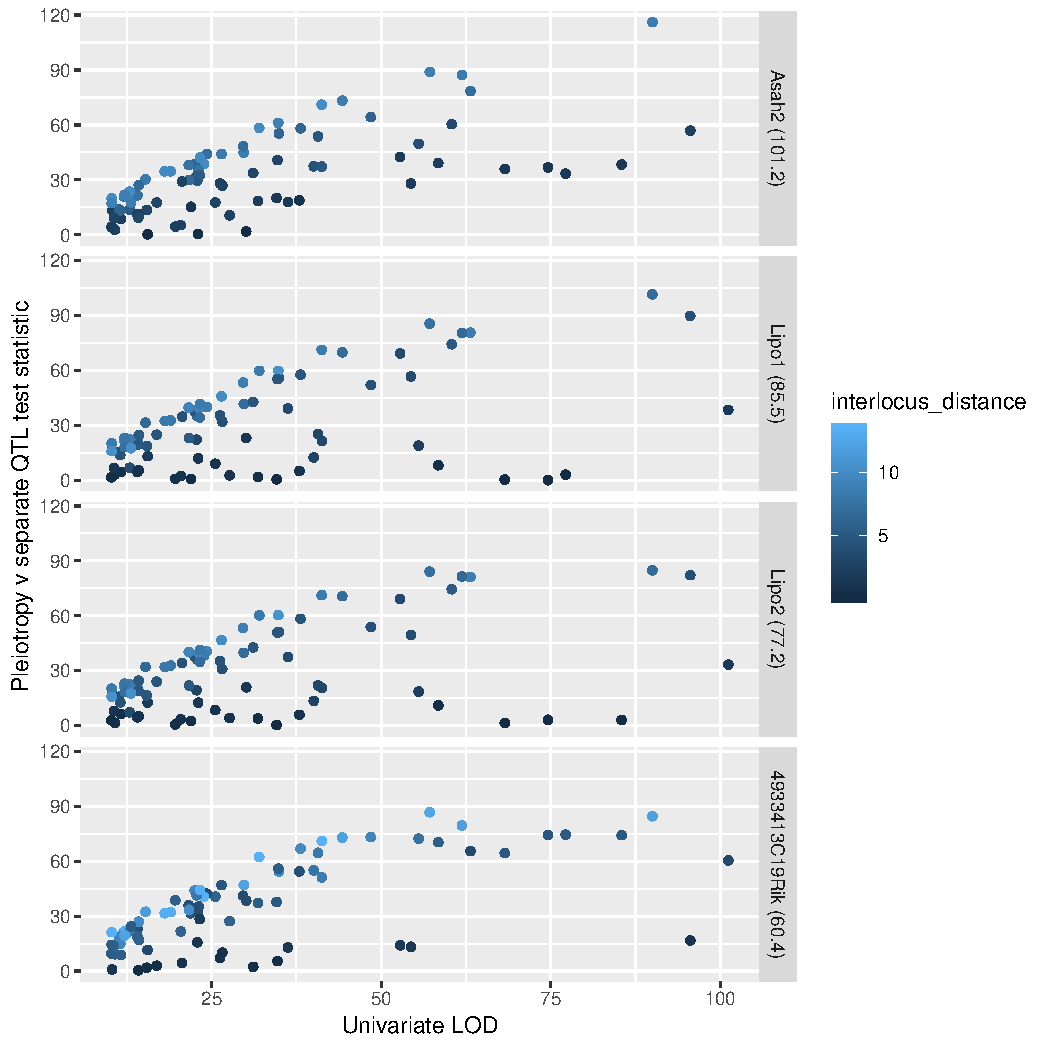
\includegraphics[width = \textwidth]{../Rmd/lrt-v-univariate-lod.pdf}
    \caption[Pleiotropy LRT vs. univariate LOD score plots reveal that greater univariate LOD scores (and greater interlocus distance) tend to correspond to greater pleiotropy LRT values.]{Vertical axis denotes pleiotropy test statistic value, while horizontal axis denotes univariate LOD score. Each point corresponds to a single gene expression trait. Panels correspond to the anchor gene expression trait. The pleiotropy test statistics correspond to analyses involving a single gene expression trait and the specified anchor gene expression trait.}
    \label{fig:lod}
\end{figure}

Analyses for all four anchor gene expression traits demonstrate that greater univariate LOD scores tend to correspond to greater values of the pleiotropy test statistic (Figure \ref{fig:lod}).








%\subsection{Pleiotropy likelihood ratio test statistics vs. fitted values correlation}

\begin{figure}
    \centering
    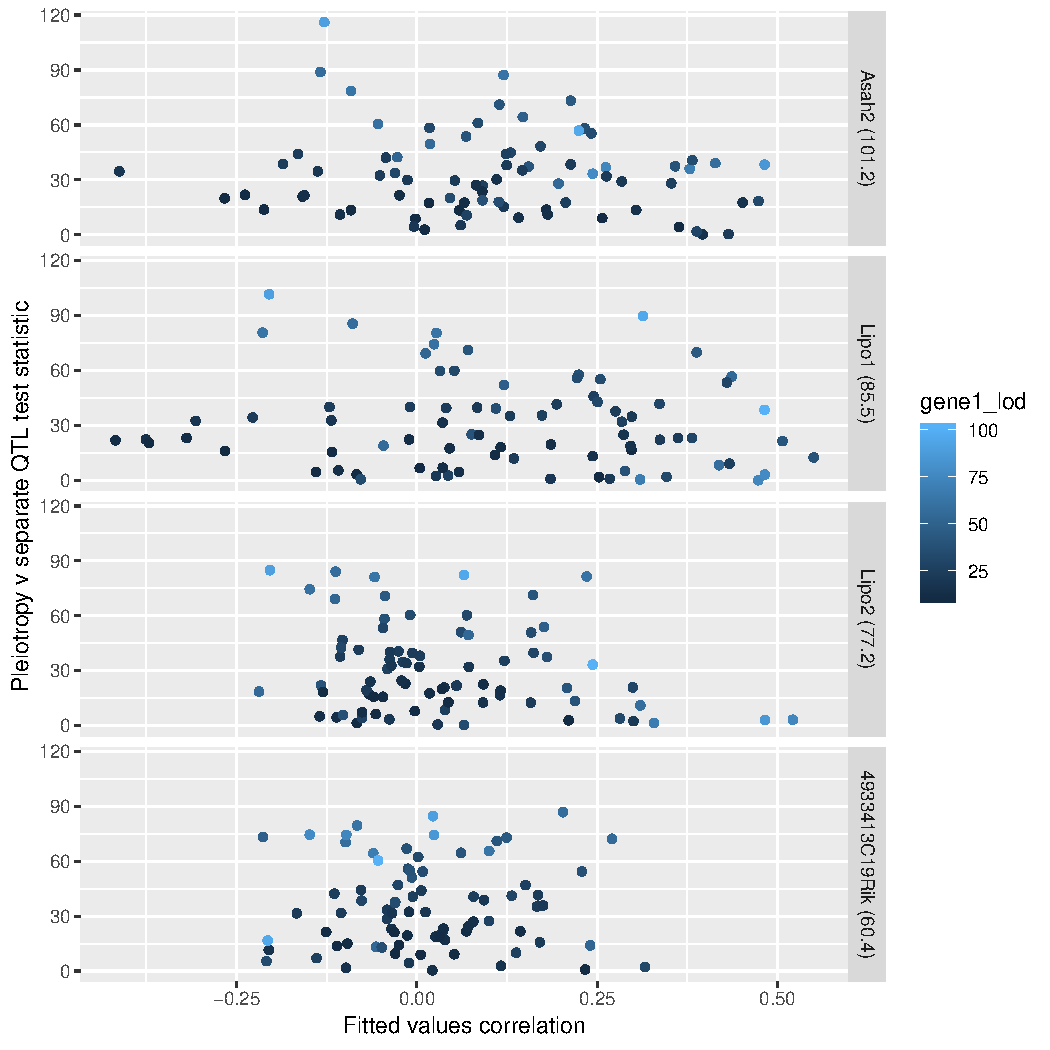
\includegraphics[width = \textwidth]{../Rmd/lrt-v-corr.pdf}
    \caption[Pleiotropy LRT vs. fitted values correlations plots reveal little evidence for a relationship.]{Vertical axis denotes the pleiotropy test statistic value, and horizontal axis indicates absolute value of the correlation between vectors of fitted values. Each point corresponds to a pairing between the specified anchor expression trait and one of the 79 other expression traits.}
    \label{fig:cor}
\end{figure}

Figure \ref{fig:cor} features four panels, one for each anchor gene. Each point corresponds to a pairing between the specified anchor and one of the 79 other gene expression traits.



\section{Discussion}

Our goal for this study was to characterize the impacts of univariate LOD score, inter-locus distance, and founder allele effects pattern similarities on pleiotropy test statistic values. Our study design, in which we examined 310 pairs of local gene expression traits on Chromosome 19, allowed us to interrogate both the effects of univariate association strength and the effects of inter-locus distance. We found that stronger univariate associations and greater inter-locus distances correspond to greater pleiotropy test statistic values (Figures \ref{fig:middle} and \ref{fig:lod}). We expected these trends based on our simulation studies in Chapter 2.

Figure \ref{fig:cor} revealed no marginal relationship between fitted values correlations and pleiotropy test statistics. However, close examination of Figure \ref{fig:cor} reveals the possibility that there is an interaction between 1) fitted values correlations and 2) univariate association strength. In every panel, those expression traits with stronger univariate associations tend to have steeper slopes between the conditional mean pleiotropy test statistic values and fitted values correlations. The plots suggest that, at greater univariate LOD values, there is a greater (negative) relationship between fitted values correlation and pleiotropy test statistic value.

We anticipated that more similar founder allele effects patterns would correspond to smaller values for the pleiotropy test statistic, when holding other factors constant. As we stated above, \citet{macdonald2007joint} and \citet{king2012genetic} argued that, for biallelic markers, two pleiotropic traits should have similar founder allele effects patterns. In our setting, it's unclear whether the markers are biallelic in the collection of eight founder lines.

We've demonstrated strong evidence in support of the roles of 1) univariate QTL LOD scores and 2) interlocus distances impacting pleiotropy test statistic values. Greater univariate QTL scores and greater interlocus distance lead to greater pleiotropy test statistics. Future research may clarify the impoact of founder allele effects patterns on pleiotropy test statistics. The fact that all four anchor traits had strong PWK effects limited our ability to fully define the impact of allele effects patterns on our test statistics.

Throughout this study, we elected to use test statistic values rather than p-values, as our measure of evidence supporting the separate QTL hypothesis. The primary reason for doing this is to avoid the computationally costly bootstrap sampling and two-dimensional QTL scans that we would need to get bootstrap p-values.

We share our analysis \texttt{R} code \citep{r} as a \texttt{git} repository at this URL: \url{https://github.com/fboehm/keller-2018-chr19-power}.

\end{boehm}

\begin{boehm}
% latex table generated in R 3.5.2 by xtable 1.8-3 package
% Thu Jan  3 16:43:33 2019
\begin{table}[ht]
\caption{Annotations for 76 non-anchor genes on Chromosome 19.}\label{tab:ann76}
\centering
\begingroup\tiny
\begin{tabular}{>{\em}lrrrr}
  \hline
Gene & Start & End & Peak position & LOD \\
  \hline
C030046E11Rik & 29.52 & 29.61 & 29.55 & 95.58 \\
  Tctn3 & 40.60 & 40.61 & 40.59 & 90.00 \\
  Gm7237 & 33.41 & 33.42 & 33.67 & 74.61 \\
  Lipo4 & 33.50 & 33.52 & 34.00 & 68.23 \\
  Dock8 & 25.00 & 25.20 & 25.07 & 63.17 \\
  Sorbs1 & 40.30 & 40.40 & 40.48 & 61.89 \\
  Lipm & 34.10 & 34.12 & 34.06 & 58.43 \\
  Blnk & 40.93 & 40.99 & 40.76 & 57.16 \\
  A830019P07Rik & 35.84 & 35.92 & 35.60 & 55.54 \\
  Uhrf2 & 30.03 & 30.09 & 29.96 & 54.40 \\
  Mbl2 & 30.23 & 30.24 & 30.18 & 52.81 \\
  Myof & 37.90 & 38.04 & 38.05 & 48.46 \\
  Gm27042 & 40.59 & 40.59 & 40.61 & 44.27 \\
  Btaf1 & 36.93 & 37.01 & 36.90 & 41.25 \\
  Hoga1 & 42.05 & 42.07 & 42.09 & 41.23 \\
  Ppp1r3c & 36.73 & 36.74 & 36.53 & 40.69 \\
  Pcgf5 & 36.38 & 36.46 & 36.24 & 40.06 \\
  Slc35g1 & 38.40 & 38.41 & 38.35 & 38.11 \\
  Pten & 32.76 & 32.83 & 32.77 & 37.95 \\
  Gldc & 30.10 & 30.18 & 30.17 & 36.26 \\
  Lgi1 & 38.26 & 38.31 & 38.17 & 34.91 \\
  C330002G04Rik & 23.04 & 23.08 & 23.34 & 34.84 \\
  Ppapdc2 & 28.96 & 28.97 & 29.09 & 34.71 \\
  Gm8978 & 33.61 & 33.63 & 33.03 & 34.59 \\
  Mms19 & 41.94 & 41.98 & 41.98 & 32.03 \\
  Ankrd22 & 34.12 & 34.17 & 34.04 & 31.83 \\
  Cdc37l1 & 28.99 & 29.02 & 29.03 & 31.14 \\
  Sgms1 & 32.12 & 32.39 & 32.11 & 30.10 \\
  Entpd1 & 40.61 & 40.74 & 40.50 & 29.73 \\
  Cbwd1 & 24.92 & 24.96 & 24.73 & 29.65 \\
  Gm14446 & 34.59 & 34.60 & 34.28 & 27.65 \\
  Ermp1 & 29.61 & 29.65 & 29.70 & 26.57 \\
  Gm9938 & 23.72 & 23.73 & 23.87 & 26.46 \\
  Insl6 & 29.32 & 29.33 & 29.37 & 26.23 \\
  Slc16a12 & 34.67 & 34.75 & 34.71 & 25.54 \\
  Pgm5 & 24.68 & 24.86 & 25.00 & 24.30 \\
  Morn4 & 42.07 & 42.09 & 41.79 & 23.86 \\
  Exosc1 & 41.92 & 41.93 & 42.10 & 23.28 \\
  Smarca2 & 26.61 & 26.78 & 26.59 & 23.25 \\
  4930418C01Rik & 24.42 & 24.43 & 23.92 & 23.10 \\
  2700046G09Rik & 32.39 & 32.39 & 32.25 & 23.02 \\
  Kcnv2 & 27.32 & 27.34 & 27.14 & 22.88 \\
  1500017E21Rik & 36.61 & 36.71 & 37.07 & 22.78 \\
  Fra10ac1 & 38.19 & 38.22 & 38.35 & 22.48 \\
  Rnls & 33.14 & 33.39 & 34.17 & 21.94 \\
  Noc3l & 38.79 & 38.82 & 40.20 & 21.67 \\
  Pip5k1b & 24.29 & 24.56 & 24.15 & 21.62 \\
  Plgrkt & 29.35 & 29.37 & 29.37 & 20.65 \\
  Ifit3 & 34.58 & 34.59 & 34.28 & 20.45 \\
  Fas & 34.29 & 34.33 & 34.20 & 19.65 \\
  Slit1 & 41.60 & 41.74 & 41.70 & 18.95 \\
  Rrp12 & 41.86 & 41.90 & 41.71 & 18.09 \\
  Ak3 & 29.02 & 29.05 & 29.55 & 16.90 \\
  A1cf & 31.87 & 31.95 & 32.11 & 15.56 \\
  4430402I18Rik & 28.90 & 28.97 & 29.37 & 15.43 \\
  Pdlim1 & 40.22 & 40.27 & 40.25 & 15.25 \\
  Gm26902 & 34.47 & 34.48 & 36.15 & 14.26 \\
  Plce1 & 38.48 & 38.79 & 38.42 & 14.26 \\
  Slc1a1 & 28.84 & 28.91 & 28.97 & 14.18 \\
  Fam122a & 24.48 & 24.48 & 24.08 & 14.07 \\
  Lipa & 34.49 & 34.53 & 34.29 & 14.06 \\
  Mamdc2 & 23.30 & 23.45 & 23.35 & 13.12 \\
  Kif11 & 37.38 & 37.42 & 37.33 & 12.93 \\
  4933411K16Rik & 42.05 & 42.05 & 42.08 & 12.92 \\
  Ccnj & 40.83 & 40.85 & 40.59 & 12.19 \\
  Gm340 & 41.58 & 41.59 & 41.30 & 12.17 \\
  Fxn & 24.26 & 24.28 & 24.31 & 12.07 \\
  Stambpl1 & 34.19 & 34.24 & 34.28 & 11.62 \\
  Pde6c & 38.13 & 38.18 & 38.07 & 11.54 \\
  Cyp26a1 & 37.70 & 37.70 & 37.48 & 11.35 \\
  Ch25h & 34.47 & 34.48 & 32.50 & 10.74 \\
  Pank1 & 34.81 & 34.88 & 35.55 & 10.61 \\
  9930021J03Rik & 29.71 & 29.81 & 28.71 & 10.32 \\
  Klf9 & 23.14 & 23.17 & 23.34 & 10.26 \\
  Ubtd1 & 41.98 & 42.03 & 41.71 & 10.25 \\
  Lipk & 34.01 & 34.05 & 34.29 & 10.23 \\
   \hline
\end{tabular}
\endgroup
\end{table}

\end{boehm}

\end{document}
